% LTeX: language=en-US
\section{The Perturbation Approach}

\subsection{The Idea}
\renewcommand{\Source}{\textcite{Judd1998}, Ch. 13}
\begin{frame}{The idea of regular perturbation}
  \begin{witemize}
    \item Consider problem that reduces to solving
          \begin{equation}
            f\left( {x,\varepsilon } \right) = 0
          \end{equation}
          for variable $x$ and a parameter $\varepsilon$
    \item Assume each value for $\varepsilon$, equation has solution for $x$\\
          $\rightarrow$ set of equations in $x$ parameterized by $\varepsilon$
    \item Let $x(\varepsilon)$ be smooth function of $\varepsilon$:
          \begin{equation}
            f\left( {x\left( \varepsilon  \right),\varepsilon } \right) = 0 \label{eq:pert_basic}
          \end{equation}
    \item Goal: find $x\left( \varepsilon  \right)$
    \item Generally impossible to solve \eqref{eq:pert_basic} for arbitrary $\varepsilon$, but may be possible for special $\varepsilon$
  \end{witemize}
\end{frame}


\begin{frame}{Simple example}
  \begin{itemize}
    \item Assume $x(0)$ is known and use implicit differentiation in univariate/scalar case:
          \begin{equation}
            {f_x }\left( {x\left( \varepsilon  \right),\varepsilon } \right){x_\varepsilon }\left( \varepsilon  \right) + {f_\varepsilon}\left( {x\left( \varepsilon  \right),\varepsilon } \right) = 0
          \end{equation}
    \item Equation implicitly defines derivative $x_\varepsilon\left( \varepsilon  \right)$
    \item Problem: still depends on unknown $x\left( \varepsilon  \right)$
    \item Evaluating at $\varepsilon=0$ yields
          \begin{equation}
            {f_x}\left( {x\left( 0 \right),0} \right){x_\varepsilon }\left( 0 \right) + {f_\varepsilon }\left( {x\left( 0 \right),0} \right) = 0
          \end{equation}
          which implies
          \begin{equation}
            {x_\varepsilon }\left( 0 \right) =  - \frac{{{f_\varepsilon }\left( {x\left( 0 \right),0} \right)}}{{{f_x}\left( {x\left( 0 \right),0} \right)}}
          \end{equation}
    \item Given we know $x(0)$ and function $f$, we can compute $x_\varepsilon\left( 0 \right)$ and get the linear approximation
          \begin{equation}
            {x }\left( \varepsilon \right) =x(0)  - \frac{{{f_\varepsilon }\left( {x\left( 0 \right),0} \right)}}{{{f_x}\left( {x\left( 0 \right),0} \right)}}(\varepsilon-0)
          \end{equation}
  \end{itemize}
\end{frame}


\begin{frame}{Continuing the simple example}
  \begin{itemize}
    \item Differentiating a second time yields
          \begin{align}
            0= & {f_{xx}}\left( {x\left( \varepsilon  \right),\varepsilon } \right){\left( {{x_\varepsilon }\left( \varepsilon  \right)} \right)^2} + 2{f_{x\varepsilon }}\left( {x\left( \varepsilon  \right),\varepsilon } \right){x_\varepsilon }\left( \varepsilon  \right) \notag \\
               & + {f_x}\left( {x\left( \varepsilon  \right),\varepsilon } \right){x_{\varepsilon \varepsilon }}\left( \varepsilon  \right) + {f_{\varepsilon \varepsilon }}\left( {x\left( \varepsilon  \right),\varepsilon } \right)
          \end{align}
    \item This implies
          \hspace{-0.5cm}
          \begin{align*}
             & {x_{\varepsilon \varepsilon }}\left( 0 \right)= (-1)\times                                                                                                                                                                                                                                                    \\
             & \frac{{{f_{xx}}\left( {x\left( 0 \right),0} \right){{x_\varepsilon^2 }\left( 0 \right)} + 2{f_{x\varepsilon }}\left( {x\left( 0 \right),0} \right){x_\varepsilon }\left( 0 \right) + {f_{\varepsilon \varepsilon }}\left( {x\left( 0 \right),0} \right)}}{{{f_x}\left( {x\left( 0 \right),0} \right)}} \notag
          \end{align*}
    \item Evaluating at 0 yields:
          \begin{equation}
            x\left( \varepsilon  \right) = x\left( 0 \right) - {x_\varepsilon }\left( 0 \right)\left( {\varepsilon  - 0} \right) - \frac{1}{2}{x_{\varepsilon \varepsilon }}\left( 0 \right){\left( {\varepsilon  - 0} \right)^2}
          \end{equation}
    \item As long as there are sufficient derivatives of $f$, we can continue
    \item Each successive differentiation results in a linear equation for the next derivative of $x(\varepsilon)$
    \item Effectively, \highlight{we construct our solution from a point that we know a lot about}, usually the deterministic steady state
  \end{itemize}
\end{frame}
\note{
  The first term uses the product rule for both arguments so that four terms arise
  \[\begin{gathered}
      {f_{xx}}\left( {x\left( \varepsilon  \right),\varepsilon } \right){\left( {{x_\varepsilon }\left( \varepsilon  \right)} \right)^2} + {f_x}\left( {x\left( \varepsilon  \right),\varepsilon } \right) \times 0 \hfill \\
      + {f_{x\varepsilon }}\left( {x\left( \varepsilon  \right),\varepsilon } \right){x_\varepsilon }\left( \varepsilon  \right) + {f_x}\left( {x\left( \varepsilon  \right),\varepsilon } \right){x_{\varepsilon \varepsilon }}\left( \varepsilon  \right) \hfill \\
      + {f_{\varepsilon x}}\left( {x\left( \varepsilon  \right),\varepsilon } \right){x_\varepsilon }\left( \varepsilon  \right) + {f_{\varepsilon \varepsilon }}\left( {x\left( \varepsilon  \right),\varepsilon } \right) = 0 \hfill \\
    \end{gathered} \]
}

\begin{frame}{Singular perturbation}
  \begin{itemize}
    \item The example up to this point considered \highlight{regular perturbation}, but we are typically interested in stochastic problems that depend on shocks $\nu_t$:
          \begin{equation}
            E_t f\left( {{x_t},{\nu _t}} \right) = 0
          \end{equation}
    \item But we only know the solution at the deterministic steady state, i.e.\ in the deterministic case with
          \begin{equation}
            f\left( x_t,0 \right) = 0
          \end{equation}
    \item We could try to use our previous approach by writing:
          \begin{equation}
            E_t f\left( {{x_t},{\varepsilon\nu _t}} \right) = 0
          \end{equation}
          and perturbing around $\varepsilon=0$
    \item Problem: changing $\varepsilon$ from 0 to any non-zero value introduces a \highlight{singular perturbation} as it changes the order of the problem
    \item E.g.\ $x_t=\rho x_{t-1}+\varepsilon \nu_t$ would collapse to $x_t=x_{t-1}=\bar x$
  \end{itemize}
\end{frame}

\renewcommand{\Source}{}
\subsection{Regular vs. singular perturbation}
\begin{frame}{Singular perturbation}
  \begin{witemize}
    \item \textcite{Fleming1971}: we can treat this singular perturbation in $\varepsilon$ as a regular perturbation \parencite[according to][]{Judd1998}
    \item However: not completely clear, what the correct way is
    \item It looks as if \textcite{Fleming1971} first takes the derivative w.r.t.\ to the perturbation parameter and then tries to find the solution to the perturbed system
    \item Standard practice in economics is to simultaneously take the derivative w.r.t.\ to the perturbation parameter and the state variables
    \item For example, \textcite{FVetal2010b} add perturbation parameter to the state vector and treat it essentially as a state
    \item This creates a lot of issues
  \end{witemize}
\end{frame}

\begin{frame}{Example}
  \begin{itemize}
    \item Consider the problem
          \begin{equation}
            \mathop {\max }\limits_{{y_t}}  -{E_t}{\left( y_t - e^{x_t+1} \right)^2}
          \end{equation}
    \item Can be motivated by the optimization problem of a bank choosing its capital level $y_t$ for next period, while the capital requirement $e^{x_{t+1}}$ is stochastic
    \item Having more or less capital than this target level is costly
    \item Assume that the required capital follows:
          \begin{equation}
            x_{t+1}=\rho {x_t} + {\varepsilon _{t + 1}}
          \end{equation}
    \item The FOC is given by
          \begin{equation}
            y_t = {E_t}\left[ {{e^{\rho {x_t} + {\varepsilon _{t + 1}}}}} \right] \label{eq:aes_example_FOC}
          \end{equation}
          and the analytical solution by:
          \begin{equation}
            y_t = {e^{\rho {x_t} + \frac{1}{2}Var\left( {{\varepsilon _t}} \right)}} \label{eq:aes_example_true_solution}
          \end{equation}
  \end{itemize}
\end{frame}

\begin{frame}{Singular and regular perturbation simultaneously}
  \begin{itemize}
    \item Take the FOC
          \begin{equation}
            y_t = {E_t}\left[ {{e^{\rho {x_t} + \sigma{\varepsilon _{t + 1}}}}} \right] \tag{\ref{eq:aes_example_FOC}}
          \end{equation}
          and perform a Taylor approximation w.r.t.\ $x_t$ and $\sigma$ about the deterministic steady state $(0,0)$
          \begin{align}
            {y_t} & \approx {E_t}\left[ {1 + {e^0}\rho \left( {{x_t} - 0} \right) + {e^0}{\varepsilon _{t + 1}}\left( {\sigma  - 0} \right)} \right] \notag \\
                  & = 1 + \rho {x_t}
          \end{align}
    \item Good approximation to the true solution if system is deterministic, i.e.\ $Var\left( {{\varepsilon _t}} \right)=0$
    \item Solution is certainty equivalent (as opposed to the true solution/problem)
  \end{itemize}
\end{frame}

\renewcommand{\Source}{\textcite{Evers2012}}
\begin{frame}{Singular perturbation first}
  \begin{itemize}
    \item Example follows the procedure advocated by \textcite{Evers2012}
    \item Take the FOC
          \begin{equation}
            y_t = {E_t}\left[ {{e^{\rho {x_t} + \sigma{\varepsilon _{t + 1}}}}} \right] \tag{\ref{eq:aes_example_FOC}}
          \end{equation}
          and perform a second order Taylor approximation w.r.t.\ $\sigma$ about the deterministic steady model ($\sigma=0$):
          \begin{align}
            {y_t} & \approx {E_t}\left[ {{e^{\rho {x_t}}} + {e^{\rho {x_t}}}{\varepsilon _{t + 1}}\left( {\sigma  - 0} \right) + {e^{\rho {x_t}}}\varepsilon _{t + 1}^2{{\left( {\sigma  - 0} \right)}^2}} \right] \notag                \\
                  & = {e^{\rho {x_t}}} + \frac{1}{2}{e^{\rho {x_t}}}{\sigma ^2}{E_t}\varepsilon _{t + 1}^2 \notag                                                                                                                        \\
                  & = {e^{\rho {x_t}}} + \frac{1}{2}{e^{\rho {x_t}}}Var_t\left( {{\varepsilon _{t+1}}} \right) =  {e^{\rho {x_t}}} + \frac{1}{2}{e^{\rho {x_t}}}Var\left( {{\varepsilon _{t}}} \right) \label{eq:aes_example_aes_system}
          \end{align}
    \item This approximated equilibrium system is now deterministic, but captures the effect of stochastics via the first two moments of the distribution of exogenous shocks
  \end{itemize}
\end{frame}

\begin{frame}{Regular perturbation second}
  \begin{itemize}
    \item Then take the approximated equilibrium system
          \begin{equation}
            y_t \approx {e^{\rho {x_t}}} + \frac{1}{2}{e^{\rho {x_t}}}Var\left( {{\varepsilon _t}} \right) \tag{\ref{eq:aes_example_aes_system}}
          \end{equation}
    \item Perform Taylor approximation w.r.t.\ the state variable $x_t$ about the deterministic steady state $x_t=0$:
          \begin{align}
            {y_t} & \approx 1 + \frac{1}{2}Var\left( {{\varepsilon _t}} \right) + \rho {e^0}\left( {{x_t} - 0} \right) + \frac{1}{2}\rho {e^0}Var\left( {{\varepsilon _t}} \right)\left( {{x_t} - 0} \right) \notag \\
                  & = 1 + \frac{1}{2}Var\left( {{\varepsilon _t}} \right) + \rho \left( {1 + \frac{1}{2}Var\left( {{\varepsilon _t}} \right)} \right){x_t}
          \end{align}
    \item Compare this with the true solution
          \begin{equation}
            y_t = {e^{\rho {x_t} + \frac{1}{2}Var\left( {{\varepsilon _t}} \right)}} \tag{\ref{eq:aes_example_true_solution}} \: ,
          \end{equation}
          whose first order approximation about $x_t=\bar x=0$ is given by
          \begin{equation}
            {y_t} \approx {e^{\frac{1}{2}Var\left( {{\varepsilon _t}} \right)}} + {e^{\frac{1}{2}Var\left( {{\varepsilon _t}} \right)}}\rho {x_t}
          \end{equation}
    \item Stochastics should affect the mean and the slope!
  \end{itemize}
\end{frame}

\begin{frame}{Regular perturbation second}
  \begin{figure}
    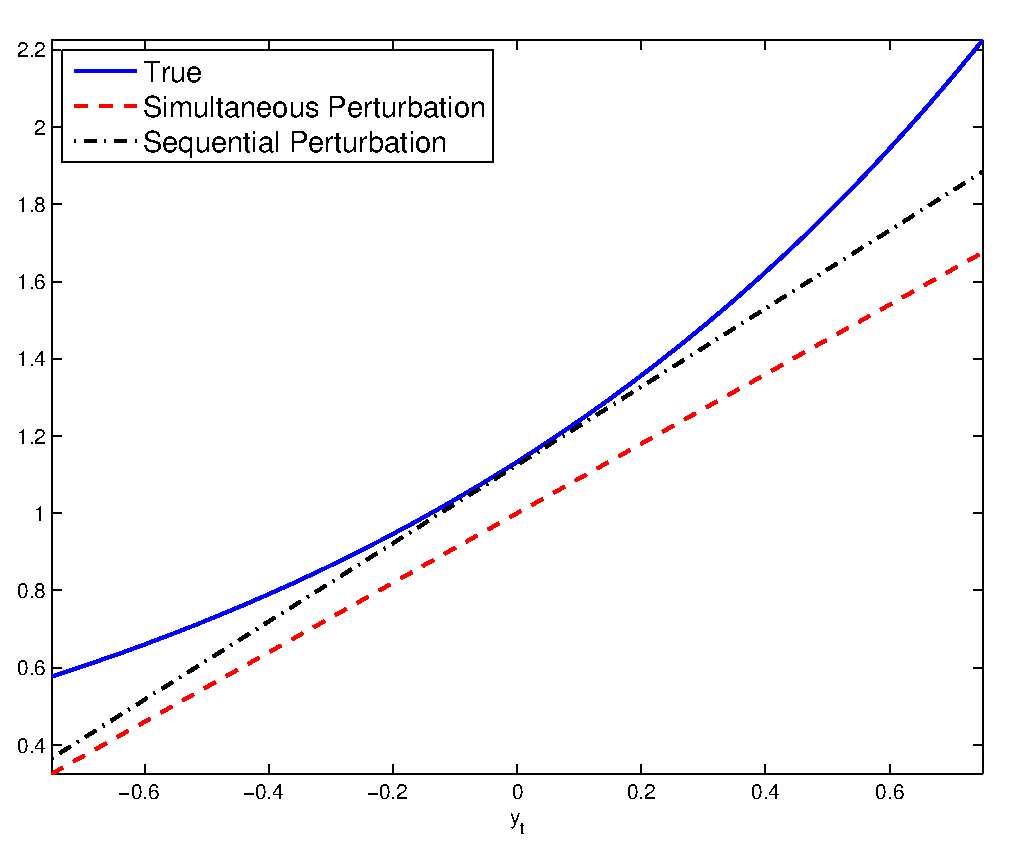
\includegraphics[scale=0.4]{AES_example}
    \caption{$\rho=0.9,\text{Var}(\varepsilon_t)=0.25$}
  \end{figure}
  \begin{itemize}
    \item But the simultaneous perturbation neglects the stochastics and results in both a mean shift and an error in the slope
  \end{itemize}
\end{frame}

\begin{frame}{Path dependency and the literature}
  \begin{witemize}
    \item Various papers have tried to solve this issue \parencite[e.g.][]{JuillardKamenik2005,Coeurdacier2011,LanMeyerGohde2013decomposing,LanMeyerGohde2013movingaverage}
    \item But none of these approaches has become the standard for various reasons
  \end{witemize}
\end{frame}



\section{Higher-order perturbation}
\subsection{Introduction}
\renewcommand{\Source}{}
\begin{frame}{Back to the literature on second-order perturbation}
  \begin{witemize}
    \item \textcite{SGU2004} is the standard reference, but thanks to Ken Judd uses horrible tensor notation
    \item \textcite{GommeKlein2011} is more accessible due to \textcite{MagnusNeudecker2007} matrix algebra
    \item We are going to follow \textcite{SGU2004}, while abusing their notation to mimic a univariate case
  \end{witemize}
\end{frame}

\renewcommand{\Source}{\textcite{SGU2004}}
\begin{frame}{The setup}
  \begin{itemize}
    \item The equilibrium conditions of many economic models can be written as
          \begin{equation}
            {E_t}\left[ {f\left( {{y_{t + 1}},{y_{t}},{x_{t+1}},{x_t}} \right)} \right] = 0 \: , \label{eq:EQ_system}
          \end{equation}
          where
          \begin{itemize}
            \item $x_t$ is an $n_x \times 1$ vector of state variables (beginning of period stock)
            \item $y_t$ is an $n_y \times 1$ vector of non-state variables (including controls)
            \item $f:{\mathbb{R}^{2{n_x} + 2{n_y}}} \to {\mathbb{R}^{{n_x} + {n_y}}}$
          \end{itemize}
    \item The system in \eqref{eq:EQ_system} together with the transversality condition implicitly defines a solution of the form
          \begin{align}
            {y_t}       & = g\left( {{x_t},\sigma } \right) \label{eq:solution_obs_eq}                                             \\
            {x_{t + 1}} & = h\left( {{x_t},\sigma } \right) + \sigma {\varepsilon _{t + 1}} \label{eq:solution_transition_eq} \: ,
          \end{align}
          where
          \begin{itemize}
            \item $\varepsilon _{t}\overset{iid}{\sim}\mathcal{N}(0,\Sigma)$
            \item $\sigma $ is the \highlight{perturbation parameter}
          \end{itemize}
    \item Note: \eqref{eq:solution_obs_eq}-\eqref{eq:solution_transition_eq} form a state-space system
  \end{itemize}
\end{frame}


\begin{frame}{Repetition: the perturbation parameter}
  \begin{witemize}
    \item The Perturbation Parameter is introduced to scale the effective distribution of shocks
    \item Consider AR1-process:
    \begin{equation}
      z_t=\rho z_{t-1}+\sigma \varepsilon_t
    \end{equation}
    \item With $\sigma=1$, the usual AR1-process results
    \item With $\sigma=0$, the system becomes deterministic
    \item We follow the literature and treat the perturbation parameter as a state variable, i.e.\ perform simultaneously the singular and regular perturbation
    %\item There is some discussion whether the perturbation parameter should scale the whole sequence of shocks from $t=-\infty$ or only from $t+1$ to $t=\infty$ \parencite[see][for the former]{Lombardo2010}
  \end{witemize}
\end{frame}

\begin{frame}{The approximation point}
  \begin{itemize}
    \item The approximation is conducted around the \highlight{deterministic steady state} characterized by $\sigma=0$, ${x_{t + 1}} = {x_t} = \bar x$ and ${y_{t + 1}} = {y_t} = \bar y$ so that
          \[
            f\left( {\bar y,\bar y,\bar x,\bar x} \right) = 0
          \]
    \item As we can express variables in deviation from their steady states, we can assume that $\bar x=\bar y=0$
  \end{itemize}
\end{frame}

\begin{frame}{A useful definition}
  \begin{itemize}
    \item For arbitrary functions $\tilde g, \tilde h$ define
          \begin{align}
             & z\left( {{x_t},\sigma ;\tilde g,\tilde h} \right)                                                                                                                                                                                                                      \\
             & = {E_t}\left[ f\left(\tilde g\left( {\tilde h\left( {{x_t},\sigma } \right) + \sigma {\varepsilon _{t + 1}},\sigma } \right),\tilde g\left( {{x_t},\sigma } \right),\tilde h\left( {{x_t},\sigma } \right) + \sigma {\varepsilon _{t + 1}},{x_t}\right) \right] \notag
          \end{align}
    \item The exact solution by definition satisfies
          \begin{equation}
            z\left( {x_t},\sigma ;g, h \right) = 0 \label{eq:exact_solution}
          \end{equation}
  \end{itemize}
\end{frame}

\begin{frame}{The central idea}
  \begin{itemize}
    \item The equilibrium conditions
          \begin{align}
            F\left( {{x_t},\sigma } \right) & \equiv {E_t}\left[ f\left(g\left( {h\left( {{x_t},\sigma } \right) + \sigma {\varepsilon _{t + 1}},\sigma } \right),g\left( {{x_t},\sigma } \right),h\left( {{x_t},\sigma } \right) + \sigma {\varepsilon _{t + 1}},{x_t}\right) \right] \notag \\
                                            & = 0
          \end{align}
          have to hold for all values of the states $x_t$
    \item Thus: \highlight{all partial derivatives with respect to the states have to be 0:}
          \begin{equation}
            {F_{{x^k},{\sigma ^j}}}\left( {{x_t},\sigma } \right) = 0 \: \forall \:  {x_t},\sigma ,j,k \: ,
          \end{equation}
          where the subscripts indicate the $k$th derivative w.r.t $x_t$ and the $j$th derivative w.r.t.\ $\sigma$
  \end{itemize}
\end{frame}

\subsection{First-order approximation}
\begin{frame}{Guess and verify}
  \begin{itemize}
    \item We proceed by using a \highlight{guess-and-verify} strategy
    \item The second-order Taylor approximation to the solution for a univariate case will take the form:
          \begin{align}
            \hat g\left( {{x_t}} \right) = {g_x}{x_t} + {g_\sigma }\sigma  +\frac{1}{2}\left[ {g_{\sigma \sigma }}{\sigma ^2} + {g_{xx}}x_t^2 + 2{g_{x\sigma }}{x_t}\sigma \right] \label{eq:g_fun} \\
            \hat h\left( {{x_t}} \right) = {h_x}{x_t} + {h_\sigma }\sigma  +\frac{1}{2}\left[ {h_{\sigma \sigma }}{\sigma ^2} + {h_{xx}}x_t^2 + 2{h_{x\sigma }}{x_t}\sigma  \right] \label{eq:h_fun}
          \end{align}
    \item The multivariate case requires more heavy notation, see \textcite{GommeKlein2011}
    \item This second order approximation can be characterized by making sure that the first two derivatives of \eqref{eq:exact_solution} are 0, i.e.\
          \[\begin{gathered}
              Dz\left( {0,0;\hat g,\hat h} \right) = 0 \hfill \\
              Hz\left( {0,0;\hat g,\hat h} \right) = 0 \hfill \\
            \end{gathered} \]
    \item Will result in a recursive structure: first solve for first order terms, then for second order terms, etc.
          %\item In principle, we already know how to solve for first-order terms
  \end{itemize}
\end{frame}


\begin{frame}{Computing  $F_x$}
  \begin{itemize}
    \item Taking the derivative w.r.t. to $x_t$ yields:
          \begin{equation}
            {F_x}\left( {\bar x,0} \right) = {f_{{y_{t + 1}}}}\left( {\bar x,0} \right){g_x}{h_x} + {f_{{y_t}}}\left( {\bar x,0} \right){g_x} + {f_{{x_{t + 1}}}}\left( {\bar x,0} \right){h_x} + {f_{x_t}}\left( {\bar x,0} \right)=0
          \end{equation}
    \item All the derivatives of $f$ evaluated at the steady state are known
    \item Unknowns are the partial derivatives $g_x$ and $h_x$
    \item Looks easy in the univariate case, but we are actually talking about $n\times n_x$ matrices where entry $i,j$ is given by
          \begin{equation}
            \left[ {{f_{{y_{t + 1}}}}\left( {\bar x,0} \right){g_x}{h_x}} \right]_i^j = \sum\limits_{\alpha  = 1}^{{n_y}} {\sum\limits_{\beta  = 1}^{{n_x}} {\frac{{\partial {f^i}}}{{\partial {y_{t + 1}}}}\frac{{\partial {g^\alpha }}}{{\partial {x^\beta }}}\frac{{\partial {h^\beta }}}{{\partial {x_j}}}} }
          \end{equation}
    \item We have a quadratic matrix equation system with $n\times n_x$ equations and $n\times n_x$ unknowns
    \item We know how to solve such a system, e.g.\ \textcite{BlanchardKahn1980} or \textcite{Klein2000}
  \end{itemize}
\end{frame}

\begin{frame}{Computing  $F_\sigma$}
  \begin{itemize}
    \item Taking the derivative w.r.t. to $\sigma$ yields:
          \begin{align}
             & {F_\sigma }\left( {\bar x,0} \right) \notag                                                                                                                                                                                                                               \\
             & = {E_t}\left[ \begin{gathered}
                                 {f_{{y_{t + 1}}}}\left( {\bar x,0} \right)\left[ {{g_x} \times \left( {{h_\sigma } + {\varepsilon _{t + 1}}} \right) + {g_\sigma }} \right] \hfill \\
                                 + {f_{{y_t}}}\left( {\bar x,0} \right){g_\sigma } + {f_{{x_{t + 1}}}}\left( {\bar x,0} \right)\left( {{h_\sigma } + {\varepsilon _{t + 1}}} \right) \hfill \\
                               \end{gathered}  \right]\notag \\
             & = {f_{{y_{t + 1}}}}\left( {\bar x,0} \right)\left[ {{g_x}{h_\sigma } + {g_\sigma }} \right] + {f_{{y_t}}}\left( {\bar x,0} \right){g_\sigma } + {f_{{x_{t + 1}}}}\left( {\bar x,0} \right){h_\sigma } \label{eq:F_sigma}
          \end{align}

    \item Again, the derivatives of $f$ evaluated at the steady state are known and so is $g_x$
    \item Thus, equation \eqref{eq:F_sigma} is a linear homogenous system of equations in $h_\sigma$ and $g_\sigma$
    \item If a unique solution exists, we must have
          \[
            {h_\sigma } = 0 \: \text{and } \: {g_\sigma } = 0
          \]
    \item This is the famous result that, at first order, the solution implies \highlight{certainty equivalence}
  \end{itemize}
\end{frame}

\subsection{Second-order solution}
\begin{frame}{Computing $F_{xx}$}
  \begin{itemize}
    \item Taking the derivative w.r.t. of $F_x$ to $x_t$ yields:
          \begin{align}
            {F_{xx}} & \left( {\bar x,0} \right) \notag                                                                                                                                \\
            =        & \left[ {f_{y_{t + 1}{y_{t + 1}}}{g_x}{h_x} + {f_{{y_{t + 1}}{y_t}}}{g_x} + {f_{{y_{t + 1}}{x_{t + 1}}}}{h_x} + {f_{{y_{t + 1}}{x_t}}}} \right]{g_x}{h_x} \notag \\
                     & + f_{{y_{t + 1}}}\left( {{g_{xx}}{h_x}{h_x} + {g_x}{h_{xx}}} \right) \notag                                                                                     \\
                     & + \left[ {{f_{y_t y_{t + 1}}}{g_x}{h_x} + {f_{{y_t}{y_t}}}{g_x} + {f_{{y_t}{x_{t + 1}}}}{h_x} + {f_{{y_t}{x_t}}}} \right]{g_x} \notag                           \\
                     & + {f_{{y_t}}}{g_{xx}} \notag                                                                                                                                    \\
                     & + \left[ {{f_{x_{t + 1} y_{t + 1}}}{g_x}{h_x} + {f_{{x_{t + 1}}{y_t}}}{g_x} + {f_{{x_{t + 1}}{x_{t + 1}}}}{h_x} + {f_{{x_{t + 1}}{x_t}}}} \right]{h_x} \notag   \\
                     & + {f_{{x_{t + 1}}}}{h_{xx}} \notag                                                                                                                              \\
                     & + f_{x_t y_{t + 1}}{g_x}{h_x} + {f_{{x_t}{y_t}}}{g_x} + {f_{{x_t}{x_{t + 1}}}}{h_x} + {f_{{x_t}{x_t}}}
            \label{eq:F_xx}
          \end{align}
    \item Makes use of product and chain rule
    \item This is a $n \times n_x \times n_x$ system of linear equations in as many unknowns
  \end{itemize}
\end{frame}
\note{In fourth line, derivative is w.r.t. to $y_{t+1}$, hence we have that additional $h_x$ shows up from $g(h(x_t))$.}

\begin{frame}{$F_{\sigma x}$}
  \begin{itemize}
    \item Next: Taking the derivative w.r.t.\ to $x$ of
          \[{F_\sigma }\left( {\bar x,0} \right) = {E_t}\left[ \begin{gathered}
                {f_{{y_{t + 1}}}}\left( {\bar x,0} \right)\left[ {{g_x}{h_\sigma } + {g_x}{\varepsilon _{t + 1}} + {g_\sigma }} \right] \hfill \\
                + {f_{{y_t}}}\left( {\bar x,0} \right){g_\sigma } + {f_{{x_{t + 1}}}}\left( {\bar x,0} \right)\left( {{h_\sigma } + {\varepsilon _{t + 1}}} \right) \hfill \\
              \end{gathered}  \right]\]
    \item We have
          \begin{align}
            {F_{\sigma x}}\left( {\bar x,0} \right) = & E_t\biggl\{ {f_{{y_{t + 1}}}}\left[ {{g_{xx}}\alert{h_\sigma } + {g_x}{h_{\sigma x}} + {g_{xx}}\alert{\varepsilon _{t + 1}} + {g_{\sigma x}}{h_x}} \right] \notag \\
                                                      & + {f_{{y_t}}}{g_{\sigma x}} \notag                                                                                                                                \\
                                                      & + {f_{{x_{t + 1}}}}{h_{\sigma x}}\biggr\}=0  \: ,
          \end{align}
          where red terms are 0
    \item This is a linear homogenous system of $n \times n_x$ equations in the same number of elements
  \end{itemize}
\end{frame}

\begin{frame}{Computing $F_{\sigma x}$}
  \begin{itemize}
    \item For
          \[{F_{\sigma x}}\left( {\bar x,0} \right) = {f_{{y_{t + 1}}}}\left[ {{g_x} + {h_x}} \right]{h_{\sigma x}} + {f_{{y_t}}}{g_{\sigma x}} + {f_{{x_{t + 1}}}}{h_{\sigma x}}\]
          to hold for all $x_t$ and the solution being unique, we must have
          \begin{align}
            {h_{\sigma x}} = 0 \\
            {g_{\sigma x}} = 0
          \end{align}
    \item The volatility of the system does not affect the response to the state variables at second order
  \end{itemize}
\end{frame}

\begin{frame}{Computing $F_{\sigma\sigma}$}
  \begin{itemize}
    \item Next: Taking the derivative  w.r.t.\ to $\sigma$ of
          \[{F_\sigma }\left( {\bar x,0} \right) = {E_t}\left[ \begin{gathered}
                {f_{{y_{t + 1}}}}\left( {\bar x,0} \right)\left[ {{g_x}{h_\sigma } + {g_x}{\varepsilon _{t + 1}} + {g_\sigma }} \right] \hfill \\
                + {f_{{y_t}}}\left( {\bar x,0} \right){g_\sigma } + {f_{{x_{t + 1}}}}\left( {\bar x,0} \right)\left( {{h_\sigma } + {\varepsilon _{t + 1}}} \right) \hfill \\
              \end{gathered}  \right]\]
    \item We have
          \begin{align}
            {F_{\sigma \sigma }} = & {E_t}\biggl\{ {f_{{y_{t + 1}}}}\left[ {\underbrace { {g_x}{h_{\sigma \sigma }} + \alert{{g_{x\sigma }}{h_\sigma }} }_{\left( {{g_x}{h_\sigma }} \right)'} + \underbrace { {\left( {{g_{xx}}\left( {\alert{h_\sigma } + {\varepsilon _{t + 1}}} \right) + \alert{g_{x\sigma }}} \right){\varepsilon _{t + 1}}} }_{\left( {{g_x}{\varepsilon _{t + 1}}} \right)'} + {g_{\sigma \sigma }}} \right] \notag \\
                                   & + {f_{{y_{t + 1}} \cdot }}\left[ {{g_x}\alert{h_\sigma } + {g_x}{\varepsilon _{t + 1}} + \alert{g_\sigma }} \right] \notag                                                                                                                                                                                                                                                                             \\
                                   & + {f_{{y_t}}}{g_{\sigma \sigma }} + {f_{{y_t} \cdot }}\alert{g_\sigma } \notag                                                                                                                                                                                                                                                                                                                         \\
                                   & + {f_{{x_{t + 1}} \cdot }}\left[ {\alert{h_\sigma } + {\varepsilon _{t + 1}}} \right] \notag                                                                                                                                                                                                                                                                                                           \\
                                   & + {f_{{x_{t + 1}}}}{h_{\sigma \sigma }}\biggr\}  \: ,
          \end{align}
          where red terms are 0
  \end{itemize}
\end{frame}

\begin{frame}{Computing $F_{\sigma\sigma}$, continued}
  \begin{itemize}
    \item Evaluating the cross-derivatives of $f$ yields:
          \begin{align}
            {F_{\sigma \sigma }} = & {E_t}\biggl\{ {f_{{y_{t + 1}}}}\left[ {{g_x}{h_{\sigma \sigma }} + {g_{xx}}\varepsilon _{t + 1}^2 + {g_{\sigma \sigma }}} \right] \notag                                           \\
                                   & + \left( {{f_{{y_{t + 1}}{y_{t + 1}}}}{g_x}{\varepsilon _{t + 1}} + {f_{{y_{t + 1}}{x_{t + 1}}}}{\varepsilon _{t + 1}}} \right)\left[ {{g_x}{\varepsilon _{t + 1}}} \right] \notag \\
                                   & + {f_{{y_t}}}{g_{\sigma \sigma }} \notag                                                                                                                                           \\
                                   & + \left( {{f_{{x_{t + 1}}{y_{t + 1}}}}{g_x}{\varepsilon _{t + 1}} + {f_{{x_{t + 1}}{x_{t + 1}}}}{\varepsilon _{t + 1}}} \right)\left[ {{\varepsilon _{t + 1}}} \right] \notag      \\
                                   & + {f_{{x_{t + 1}}}}{h_{\sigma \sigma }}\biggr\}  \: ,
          \end{align}
          where
          \[
            E_t[\varepsilon_{t+1}\varepsilon_{t+1}]
          \]
          corresponds to the covariance matrix of shocks
    \item This is a system of $n$ equations in $n$ unknowns $h_{\sigma\sigma}$ and $g_{\sigma\sigma}$
  \end{itemize}
\end{frame}

\begin{frame}{The solution}
  \begin{witemize}
    \item Summarizing, we have that all odd derivatives w.r.t. to the perturbation parameter $\sigma$ are zero
    \item Thus, the second-order solution is given by
    \begin{align}
      \hat g\left( {{x_t}} \right) = {g_x}{x_t} +\frac{1}{2}\left[ {g_{\sigma \sigma }}{\sigma ^2} + {g_{xx}}x_t^2 \right] \tag{\ref{eq:g_fun}} \\
      \hat h\left( {{x_t}} \right) = {h_x}{x_t} +\frac{1}{2}\left[ {h_{\sigma \sigma }}{\sigma ^2} + {h_{xx}}x_t^2 \right] \tag{\ref{eq:h_fun}}
    \end{align}
    \item At second-order, the solution to a stochastic DSGE model of the class considered here, differs from a deterministic setup only in a constant term $0.5 g_{\sigma\sigma}\sigma^2$
  \end{witemize}
\end{frame}

\renewcommand{\Source}{\textcite{FVetal2010a}}
\begin{frame}{Stochastic volatility}
  \begin{witemize}
    \item Here, we only considered homoskedastic shocks, so \highlight{stochastic volatility} of the form
    \begin{align}
      x_t        & =\rho x_{t-1}+e^{\sigma_{t}}\nu_{t}\ ,\quad\nu_{t}\sim\mathcal{N}(0,1)                                                             \\
      \sigma_{t} & =\left(1-\rho^{\sigma}\right)\bar{\sigma}+\rho^{\sigma}\sigma_{t-1}+\eta\varepsilon_{t}\ ,\quad\varepsilon_{t}\sim\mathcal{N}(0,1)
    \end{align}
    is excluded
    \item \textcite{FVetal2010a} show that the previous results also hold true with stochastic volatility
    \item The perturbation parameter will only have coefficients different from zero in even powers
    \item Volatility shocks appear with coefficients different from zero only in the term where they are multiplied by the innovation to their own
    structural shock
    \item[$\Rightarrow$] Pure volatility shocks have no effect up to second order
  \end{witemize}
\end{frame}


\begin{frame}{Higher-order approximations}
  \begin{witemize}
    \item Previous procedure can be easily adapted to higher orders
    \item Given second order terms, third order derivatives yield linear equation system that can be easily solved
    $\rightarrow$ Dynare does this for you at arbitrary order
    \item Most important term that appears at third order: $g_{x\sigma\sigma}$
    \item Recap:
    \begin{witemize}
      \item First order: certainty equivalence
      \item Second order: constant term in policy function
      \item Third order: volatility shocks enter the policy function linearly
    \end{witemize}
  \end{witemize}
\end{frame}

\subsection{Terminology: steady states and ergodic distribution}
\renewcommand{\Source}{\textcite{Coeurdacier2011}}
\begin{frame}{The Stochastic Steady State}
  \begin{itemize}
    \item The deterministic steady state $\bar x$ is the fixed point of the deterministic model (i.e.\ in the total absence of shocks):
          \[
            f\left( {\bar y,\bar y,\bar x,\bar x},\sigma=0 \right) = 0
          \]
    \item However: in stochastic economy, even in the absence of current shocks, agents are aware of possibility of future shocks hitting the economy\\
          $\rightarrow$ will adjust their behavior to reflect this
    \item \highlight{stochastic steady state} $\tilde x,\tilde y$ is the fixed point of the stochastic model in the absence of future shocks
          \begin{equation}
            E_t\left[f\left( {\tilde y,\tilde  y,\tilde  x,\tilde  x},\sigma=1,\{\varepsilon_i\}_{i=t}^{\infty}=0 \right)\right] = 0
          \end{equation}
    \item Traditional first order approximation: both concepts coincide
    \item Not the case anymore at higher order
  \end{itemize}
\end{frame}

\begin{frame}{Stochastic steady state and ergodic mean}
  \begin{witemize}
    \item Stochastic RBC model: agents have precautionary motive\\
    $\rightarrow$ capital stock higher than in deterministic world
    \item Term $h_{\sigma\sigma}$ embeds part of the precautionary behavior of agents:
    \begin{equation}
      \hat h\left( {{x_t}} \right) = {h_x}{x_t} +\frac{1}{2}\left[ {h_{\sigma \sigma }}{\sigma ^2} + {h_{xx}}x_t^2 \right] \tag{\ref{eq:h_fun}}
    \end{equation}
    \item If started at $x_t=\bar x=0$: if there are no realized shocks, system will move away from deterministic steady state and wander to stochastic steady state
    \item Note: generally also different from \highlight{mean of the ergodic distribution}, which is the unconditional expectation of the endogenous variables
    \item If there are shock realizations, due to Jensen's Inequality and curvature in the policy function, those shock realizations (zero for the stochastic steady state) matter
  \end{witemize}
\end{frame}



